\documentclass{article}

\usepackage{PRIMEarxiv}

\usepackage[utf8]{inputenc} % allow utf-8 input
\usepackage[T1]{fontenc}    % use 8-bit T1 fonts
\usepackage{hyperref}       % hyperlinks
\usepackage{url}            % simple URL typesetting
\usepackage{booktabs}       % professional-quality tables
\usepackage{float}
\usepackage{amsfonts}       % blackboard math symbols
\usepackage{nicefrac}       % compact symbols for 1/2, etc.
\usepackage{microtype}      % microtypography
\usepackage{fancyhdr}       % header
\usepackage{graphicx}       % graphics
\graphicspath{{media/}}     % organize your images and other figures under media/ folder

% ---------------------------------------------------------------
% Additional packages used by this report
% ---------------------------------------------------------------
\usepackage{amsmath, amssymb, amsthm, mathtools}
\usepackage{bm}
\usepackage{tabularx}
\newcolumntype{L}{>{\raggedright\arraybackslash}X}
\usepackage{adjustbox}
\usepackage{tikz}
\usetikzlibrary{arrows.meta, positioning}
\usepackage[ruled,vlined,linesnumbered]{algorithm2e}
\usepackage[capitalise,noabbrev]{cleveref}
\crefname{assumption}{assumption}{assumptions}
\Crefname{assumption}{Assumption}{Assumptions}
\usepackage{todonotes}

% ---------------------------------------------------------------
% Theorem-like environments
% ---------------------------------------------------------------
\theoremstyle{definition}
\newtheorem{definition}{Definition}
\newtheorem{assumption}{Assumption}
\newtheorem{plannedresult}{Planned Result}
\crefname{plannedresult}{Planned Result}{Planned Results}

% ---------------------------------------------------------------
% Notation macros
% ---------------------------------------------------------------
\newcommand{\E}{\mathbb{E}}
\newcommand{\Prob}{\mathbb{P}}
\newcommand{\indicator}{\mathbf{1}}
\newcommand{\Regret}{\mathrm{Reg}}
\newcommand{\pihat}{\hat{\pi}}
\newcommand{\clip}{\operatorname{clip}}
\newcommand{\sigmoid}{\operatorname{sigmoid}}
\newcommand{\logit}{\operatorname{logit}}

%Header
\pagestyle{fancy}
\thispagestyle{empty}
\rhead{ \textit{ }}

% Update your Headers here
\fancyhead[LO]{CS 329 Project Idea Review}

%% Title
\title{Deciding Task Ownership from Private Evidence under Misaligned Incentives
}

\author{
  Pranjal Goyal (24110274), Ujas Shah (24110376), Harshal Kundanlal Rana (24110131), Satyakaam Mishra(24110316) \\
  Indian Institute of Technology Gandhinagar \\
}

\begin{document}
\maketitle

\begin{abstract}
\noindent Many distributed and multi-agent systems face the task-ownership problem: determining which team owns a system incident, which software modules an issue touches, or which specialist handles a user query. Central routers relying on static textual descriptions quickly become stale, whereas candidate owners possess fresh, localized evidence but often harbor misaligned incentives that distort self-reports. We study multi-agent task assignment under private, partially verifiable evidence. Candidate agents submit confidence reports grounded in local evidence, a central mechanism assigns ownership, and three incentive mechanisms discipline strategic behavior: ex-post strictly proper scoring, cross-verification audits along an interaction graph, and cooperative credit-division rules. A single signed parameter $\ell_i \in \mathbb{R}$ captures both deflection ($\ell_i > 0$, costly ownership) and acquisition ($\ell_i < 0$, empire-building). We formalize the resulting Bayesian game, establish benchmark baselines (an omniscient oracle, stale description routing, naive polling, and plurality voting), and formulate the core research questions governing assignment efficiency, regret decomposition, audit recovery, and coalition credit sharing.
\end{abstract}

\noindent \textbf{Keywords:} Multi-agent systems $\cdot$ Mechanism design $\cdot$ Proper scoring rules $\cdot$ Cooperative games $\cdot$ Calibration

\vspace{0.4cm}

\section{Introduction}

\subsection{Motivation}
Modern software and organizational workflows continuously grapple with dispatching work to the appropriate owners. During a cloud outage, an alert fires on a downstream checkout service, even though the root cause is a silent configuration update five hops upstream. Similarly, in large codebases, a bug report must be routed to the modules it impacts, and in customer support, inquiries must reach competent specialists. In each scenario, candidate owners possess private, localized evidence (execution logs, internal metrics, commit history) that cannot be gathered or parsed centrally without prohibitive communication and processing overhead.

The identical challenge surfaces in cooperative Large Language Model (LLM) architectures. Multi-agent frameworks like AutoGen~\cite{wu2023autogen} and MetaGPT~\cite{hong2024metagpt} coordinate specialized agents, typically deploying a central router that parses high-level textual profile descriptions. However, centralized description-based routing suffers from two fundamental limitations:
\begin{enumerate}
    \item \textbf{Staleness:} Roles, codebases, and agent capabilities evolve much faster than central documentation. Misrouting is exceedingly costly; in production cloud systems, misrouting incidents can inflate diagnosis time by up to an order of magnitude~\cite{gao2020scouts}.
    \item \textbf{Misaligned Strategic Incentives:} Candidate agents are not disinterested classifiers. When agents are evaluated on individual paging load, on-call burden, or operational toil, they have an incentive to \emph{deflect} responsibility. Conversely, when rewarded for owning tasks (e.g., credit for resolving bugs or claimed compute footprint), agents have an incentive to \emph{acquire} tasks. Furthermore, LLM confidence verbalizations frequently suffer from systematic overconfidence and miscalibration~\cite{xiong2024can}.
\end{enumerate}

\subsection{Approach}
We propose a middle path between rigid central routing and unmediated self-selection. Candidate owners submit quantitative reports grounded in their private local evidence. A lightweight mechanism assigns tasks according to these reports without maintaining internal models of agent capabilities, thereby avoiding the staleness trap. To counteract strategic manipulation, the mechanism couples assignment with three economic tools:
\begin{enumerate}
    \item \textbf{Ex-post Strictly Proper Scoring:} Evaluating reports against the revealed ground truth via centered Brier scoring to align probabilistic predictions.
    \item \textbf{Graph-Structured Audits:} Randomly cross-verifying reported evidence against neighboring agents on a dependency graph to deter data tampering.
    \item \textbf{Cooperative Credit Allocation:} Employing Shapley and equal-split values to allocate collective task value among assigned coalitions.
\end{enumerate}

\subsection{Related Work and Positioning}
Prior systems like \textsc{Scouts}~\cite{gao2020scouts} train gatekeeper models per team to predict incident ownership, focusing solely on prediction accuracy rather than the underlying strategic incentives. Uncoordinated voluntary claiming among symmetric agents manifests classically as the volunteer's dilemma~\cite{diekmann1985volunteer}, where costless cheap-talk fails to communicate informative signals~\cite{crawford1982strategic}. Proper scoring rules~\cite{brier1950verification,gneiting2007strictly} elicit truthful probabilities in forecasting, while mechanism-driven audits share mathematical foundations with inspection games~\cite{avenhaus2002inspection}. For multi-agent coalition games, value attribution is governed by the Shapley value~\cite{shapley1953value} and its graph-restricted counterpart, the Myerson value~\cite{myerson1977graphs}. 

Our work bridges these disparate threads into a unified mechanism-design framework that simultaneously incorporates signed misalignment, machine-learned evidence calibration, graph-based verification, and coalition ownership against an oracle social efficiency benchmark.

\subsection{Distinguishing Attributes}
\begin{itemize}
    \item \textbf{Unified Signed Misalignment:} A single signed scalar $\ell_i \in \mathbb{R}$ captures both deflection ($\ell_i > 0$) and acquisition ($\ell_i < 0$), harmonizing blame avoidance and empire-building within one model.
    \item \textbf{Calibration in Equilibrium:} We explicitly treat the miscalibration error of machine-generated beliefs as a parameter governing strategic equilibrium reports.
    \item \textbf{First-Class Coalitions:} Tasks may require multiple owners, evaluated under explicit conjunctive (all required) and disjunctive (at least one required) resolution rules.
    \item \textbf{Domain-Agnostic Formulation:} The framework applies across disparate domains, including cloud incident routing, code ownership, and multi-agent LLM query dispatch.
\end{itemize}

\subsection{Outline}
We study: \emph{How much assignment efficiency is sacrificed relative to an omniscient oracle due to misaligned agent incentives, and to what extent can proper scoring, graph audits, and cooperative credit rules recover that loss?} 
Section~\ref{sec:preliminaries} defines foundational game-theoretic concepts. Section~\ref{sec:problem_formulation} introduces the formal game, mechanisms, regret objectives, and baseline routers. Section~\ref{sec:proposed_solutions} outlines our theoretical and empirical methodology, Section~\ref{sec:Results} shows the produced and observed results, and Section~\ref{sec:contributions} summarizes team contributions.

% -----------------------------------------------------------------------------
\section{Preliminaries}
\label{sec:preliminaries}

Table~\ref{tab:notation} outlines the primary mathematical notation.

\begin{definition}[Resolution Rules]
Let $[N] = \{1, \dots, N\}$ denote the set of agents. For a task with latent required owner set $S^* \subseteq [N]$, let $A \subseteq [N]$ be the set of assigned agents.
\begin{itemize}
    \item \textbf{Conjunctive Rule:} $V_\wedge(A; S^*) = \mathbf{1}[S^* \subseteq A]$. The task is resolved if and only if \emph{every} required owner is assigned.
    \item \textbf{Disjunctive Rule:} $V_\vee(A; S^*) = \mathbf{1}[A \cap S^* \neq \emptyset]$. The task is resolved if \emph{at least one} required owner is assigned.
\end{itemize}
When $|S^*| = 1$, both rules coincide, denoted simply by $V(A; S^*)$.
\end{definition}

\begin{definition}[Strictly Proper Scoring Rule]
A scoring function $s: [0, 1] \times \{0, 1\} \to \mathbb{R}$ is strictly proper if an agent with belief $p \in [0, 1]$ uniquely maximizes expected score $\mathbb{E}_{z \sim p}[s(r, z)] = p\, s(r, 1) + (1-p)\, s(r, 0)$ by reporting honestly: $r = p$~\cite{gneiting2007strictly}. The Brier score $s(r, z) = 1 - (z - r)^2$ is strictly proper~\cite{brier1950verification}. For a public prior base rate $\pi_i^0 = \mathbb{P}(z_i = 1)$, the \textbf{centered Brier score} is:
\begin{equation}
    \tilde{s}_i(r_i, z_i) = s(r_i, z_i) - s(\pi_i^0, z_i) = 2(z_i - \pi_i^0)(r_i - \pi_i^0) - (r_i - \pi_i^0)^2.
\end{equation}
Centering preserves strict propriety (as the subtracted term is independent of $r_i$) while ensuring that an uninformative report $r_i = \pi_i^0$ yields zero expected payout.
\end{definition}

\begin{definition}[Calibration Error]
For an agent producing probability estimates $\hat{\pi} \in [0, 1]$ regarding binary outcome $z \in \{0, 1\}$, the Expected Calibration Error (ECE) is $\mathrm{ECE} = \mathbb{E}_{\hat{\pi}}[|\mathbb{P}(z = 1 \mid \hat{\pi}) - \hat{\pi}|]$, computed empirically via equal-width or equal-mass binning~\cite{guo2017calibration}.
\end{definition}

\begin{definition}[Shapley and Myerson Values]
For a cooperative game $([N], v)$ with characteristic function $v: 2^{[N]} \to \mathbb{R}$ satisfying $v(\emptyset) = 0$, the \textbf{Shapley value}~\cite{shapley1953value} of agent $i$ is:
\begin{equation}
    \psi_i(v) = \sum_{T \subseteq [N] \setminus \{i\}} \frac{|T|!\, (N - |T| - 1)!}{N!} \left[ v(T \cup \{i\}) - v(T) \right].
\end{equation}
On a communication graph $G = ([N], E)$, the \textbf{Myerson value}~\cite{myerson1977graphs} is the Shapley value of the graph-restricted game $v^G(T) = \sum_{C \in \mathcal{C}(T)} v(C)$, where $\mathcal{C}(T)$ denotes the connected components of the induced subgraph $G[T]$.
\end{definition}

% -----------------------------------------------------------------------------
\section{Problem Formulation}
\label{sec:problem_formulation}

\subsection{Tasks, Agents, and Information Boundaries}
Consider $N \ge 2$ agents interconnected via an undirected relation graph $G = ([N], E)$, where $\mathcal{N}(i)$ denotes the set of neighbors of agent $i$ and $m_i = |\mathcal{N}(i)|$. Each task is defined by a latent owner set $S^* \subseteq [N]$ drawn from a prior distribution, with binary membership indicators $z_i = \mathbf{1}[i \in S^*]$. Nature generates an evidence profile $\mathbf{e} = (e_1, \dots, e_N) \sim P(\cdot \mid S^*, G)$. Agent $i$ observes only its local private evidence $e_i$.

\begin{table}[t]
\centering
\small
\caption{Mathematical notation.}
\label{tab:notation}
\begin{tabularx}{\textwidth}{lX}
\toprule
\textbf{Symbol} & \textbf{Description} \\
\midrule
$N, [N]$ & Number of candidate agents; index set $\{1, \dots, N\}$ \\
$S^* \subseteq [N], k$ & Latent set of required owners; coalition size $k = |S^*|$ \\
$z_i = \mathbf{1}[i \in S^*]$ & Ground-truth membership indicator for agent $i$ \\
$G = ([N], E), \mathcal{N}(i), m_i$ & Interaction graph; neighborhood of agent $i$; degree $m_i = |\mathcal{N}(i)|$ \\
$e_i$ & Private evidence observed locally by agent $i$ \\
$\pi_i^*, \pi_i, \hat{\pi}_i$ & Full-info posterior $\mathbb{P}(z_i=1 \mid \mathbf{e})$; local belief $\mathbb{P}(z_i=1 \mid e_i)$; perceived estimate \\
$r_i \in [0, 1]$ & Ownership probability report submitted by agent $i$ \\
$A \subseteq [N], x_i(\mathbf{r})$ & Selected owner set; interim assignment probability $\mathbb{P}(i \in A \mid \mathbf{r})$ \\
$V(A; S^*) \in \{0, 1\}$ & Task resolution indicator under conjunctive ($V_\wedge$) or disjunctive ($V_\vee$) rules \\
$R, c_i$ & Task resolution value; public social cost of assigning agent $i$ \\
$\ell_i \in \mathbb{R}, \phi$ & Private net assignment cost ($\ell_i > 0$: deflector, $\ell_i < 0$: acquirer); misaligned fraction \\
$\lambda, \tilde{s}_i$ & Scoring rule scale parameter; centered Brier score \\
$\pi_i^0, X_i(r_i)$ & Prior base rate $\mathbb{P}(z_i = 1)$; interim assignment curve $\mathbb{E}_{\mathbf{r}_{-i}}[x_i(r_i, \mathbf{r}_{-i})]$ \\
$\alpha, \delta, q_i, F$ & Audit rate; per-neighbor exposure probability; audit detection probability; penalty \\
$\chi_i, \psi_i$ & Credit allocated to agent $i$; Shapley value share \\
$W, \mathrm{Reg}, \eta$ & Expected social welfare; regret against oracle; social efficiency ratio \\
\bottomrule
\end{tabularx}
\end{table}

\begin{table}[t]
\centering
\small
\caption{Information structure across entities.}
\label{tab:info_structure}
\begin{tabular}{lccc}
\toprule
\textbf{Quantity} & \textbf{Agent $i$} & \textbf{Mechanism} & \textbf{Ground Truth / Nature} \\
\midrule
Latent owners $S^*$ & Unknown & Unknown & Revealed ex-post \\
Local evidence $e_i$ & Known & Payload only (partially checkable) & Known \\
Peer evidence $e_{j \neq i}$ & Unknown & Payloads only & Known \\
Graph $G$, costs $c_i$, value $R$ & Known & Known & Known \\
Private cost $\ell_i$ & Known to $i$ & Unknown & Known \\
Evidence tampering flag & Known to $i$ & Detectable via audit only & Known to simulator \\
Calibration curve of $\hat{\pi}_i$ & Unknown & Inferred from historical data & Observable ex-post \\
\bottomrule
\end{tabular}
\end{table}

\begin{assumption}[Conditional Independence]
\label{ass:cond_indep}
Conditioned on evidence vector $\mathbf{e}$, indicators $z_1, \dots, z_N$ are mutually independent with full-information posterior $\mathbb{P}(z_i = 1 \mid \mathbf{e}) = \pi_i^*$. When $|S^*| = 1$ or evidence depends solely on $z_i$, this holds exactly; on coupled graphs, it serves as an analytical approximation.
\end{assumption}

\begin{assumption}[Ex-Post Verification]
\label{ass:ex_post}
The true owner set $S^*$ is revealed ex-post upon task execution (e.g., via git blame on the resolution commit or incident post-mortem logs). Evidence payloads are verifiable digital artifacts that cannot be fabricated without detection during peer cross-audits.
\end{assumption}

Each agent possesses a private cost type $\ell_i \in \mathbb{R}$: agent $i$ is a \emph{deflector} if $\ell_i > 0$, an \emph{acquirer} if $\ell_i < 0$, and \emph{aligned} if $\ell_i = 0$. A fraction $\phi \in [0, 1]$ of the agent population is misaligned ($\ell_i \neq 0$). The public social cost of assigning agent $i$ is $c_i > 0$. Table~\ref{tab:info_structure} summarizes the information boundary.

\begin{figure}[t]
\centering
\resizebox{\textwidth}{!}{%
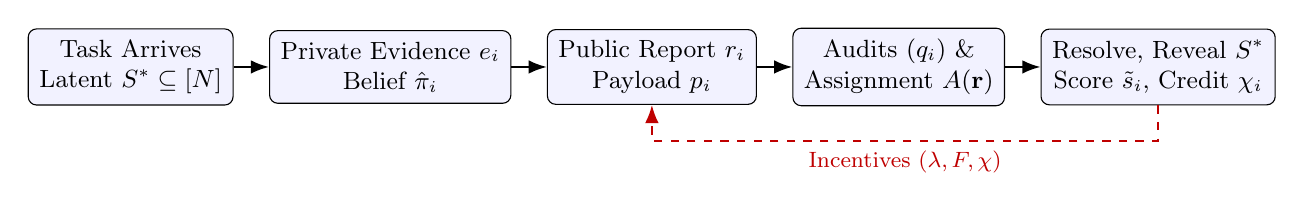
\begin{tikzpicture}[
    node distance=0.45cm,
    box/.style={draw, rounded corners=3pt, minimum height=0.85cm, align=center, font=\small, fill=blue!5, inner sep=4pt},
    arrow/.style={-Latex, thick},
    feedback/.style={-Latex, dashed, thick, color=red!75!black}
]
    \node[box] (task) {Task Arrives\\ Latent $S^* \subseteq [N]$};
    \node[box, right=of task] (evidence) {Private Evidence $e_i$\\ Belief $\hat{\pi}_i$};
    \node[box, right=of evidence] (report) {Public Report $r_i$\\ Payload $p_i$};
    \node[box, right=of report] (assign) {Audits ($q_i$) \&\\ Assignment $A(\mathbf{r})$};
    \node[box, right=of assign] (resolve) {Resolve, Reveal $S^*$\\ Score $\tilde{s}_i$, Credit $\chi_i$};

    \draw[arrow] (task) -- (evidence);
    \draw[arrow] (evidence) -- (report);
    \draw[arrow] (report) -- (assign);
    \draw[arrow] (assign) -- (resolve);

    \draw[feedback] (resolve.south) -- ++(0,-0.45) -| node[pos=0.25, below, font=\footnotesize] {Incentives $(\lambda, F, \chi)$} (report.south);
\end{tikzpicture}%
}
\caption{One assignment round. Agents control reports and payloads; the mechanism controls selection, scoring, audits, and credit allocation.}
\label{fig:round_flow}
\end{figure}

\subsection{Mechanism Rules and Agent Utilities}

\begin{definition}[Assignment Mechanism]
An assignment mechanism $\mathcal{M} = (A(\cdot), \lambda, \alpha, \chi)$ comprises a selection policy $A(\mathbf{r}) \subseteq [N]$, a scoring scale $\lambda \ge 0$, an audit rate $\alpha \in [0, 1]$, and a credit-division rule $\chi$.
\end{definition}

\noindent \textbf{Selection Rules:}
\begin{itemize}
    \item \textbf{Escalation (Disjunctive / Single-Owner Tasks):} Agents are sorted in descending order of report-to-cost ratio: $r_{(1)}/c_{(1)} \ge r_{(2)}/c_{(2)} \ge \dots \ge r_{(N)}/c_{(N)}$. Agents reporting $r_i \le 0$ are pruned. The mechanism sequentially assigns agents until the task is successfully resolved or candidate pool is exhausted.
    \item \textbf{Set Selection (Conjunctive Tasks):} Treating reports as independent posterior probabilities, the mechanism selects the coalition maximizing expected net surplus:
    \begin{equation}
        A(\mathbf{r}) \in \arg\max_{A \subseteq [N]} \left\{ R \prod_{j \notin A} (1 - r_j) - \sum_{i \in A} c_i \right\}.
    \end{equation}
\end{itemize}

\noindent \textbf{Audits and Graph Cross-Verification:}
With probability $\alpha$, the mechanism inspects agent $i$'s reported payload against its neighbors $\mathcal{N}(i)$. If agent $i$ tampered with its payload, each neighbor independently exposes an inconsistency with probability $\delta \in (0, 1)$. The overall detection probability is:
\begin{equation}
    q_i = \alpha \left[ 1 - (1 - \delta)^{m_i} \right].
\end{equation}
If detected, agent $i$ incurs a fixed penalty $F > 0$.

\noindent \textbf{Credit Rules:}
Credit is allocated exclusively to assigned agents ($i \in A$). We study:
\begin{itemize}
    \item \textbf{Equal Split:} $\chi_i^{\mathrm{equal}} = \frac{R\, V(A; S^*)}{|A|}$.
    \item \textbf{Shapley Credit:} $\chi_i^{\mathrm{shapley}} = \psi_i(v_A)$, where characteristic function $v_A(T) = R\, V(T; S^*)$ for $T \subseteq A$. Under conjunctive tasks, Shapley credit strictly rewards essential coalition members, assigning $\chi_i = 0$ to dummy agents who do not contribute to satisfying $S^* \subseteq A$.
\end{itemize}

\noindent \textbf{Agent Utility and Equilibrium:}
Agent $i$'s realized utility is:
\begin{equation}
    U_i = -\ell_i \mathbf{1}[i \in A] + \lambda \tilde{s}_i(r_i, z_i) - F \mathbf{1}[\text{tampering detected}] + \chi_i.
\end{equation}
Let $X_i(r_i) = \mathbb{E}_{\mathbf{r}_{-i}}[\mathbf{1}[i \in A(\mathbf{r})] \mid e_i, \ell_i]$ denote agent $i$'s interim assignment probability. Letting $\bar{\chi}_i = \mathbb{E}[\chi_i \mid i \in A, e_i]$ be the expected credit upon assignment, the agent faces an effective private cost $\ell_i^{\mathrm{eff}} = \ell_i - \bar{\chi}_i$. Neglecting the audit penalty term for honest payloads, the expected utility simplifies to:
\begin{equation}
    \mathbb{E}[U_i \mid e_i, \ell_i] = -\ell_i^{\mathrm{eff}} X_i(r_i) + \lambda \mathbb{E}[\tilde{s}_i(r_i, z_i) \mid e_i].
\end{equation}
Agents choose reports $r_i \in [0, 1]$ to maximize expected utility, inducing a Bayesian Nash Equilibrium.

\subsection{Objective, Oracle Benchmark, and Regret}
The expected social welfare of mechanism $\mathcal{M}$ is:
\begin{equation}
    W(\mathcal{M}) = \mathbb{E}\left[ R\, V(A; S^*) - \sum_{i \in A} c_i \right].
\end{equation}
The hypothetical full-information \textbf{Oracle} $\mathcal{M}^\circ$ observes all private evidence $\mathbf{e}$ and selects $A^\circ \in \arg\max_{A} \mathbb{E}[R V(A; S^*) - c(A) \mid \mathbf{e}]$. The performance of $\mathcal{M}$ is characterized by \textbf{Regret} and \textbf{Social Efficiency Ratio}:
\begin{equation}
    \mathrm{Reg}(\mathcal{M}) = W(\mathcal{M}^\circ) - W(\mathcal{M}) = \underbrace{R\, \mathbb{E}[V(A^\circ) - V(A)]}_{\Delta V \text{ (miss loss)}} + \underbrace{\mathbb{E}[c(A) - c(A^\circ)]}_{\Delta C \text{ (excess cost)}}, \quad \eta(\mathcal{M}) = \frac{W(\mathcal{M})}{W(\mathcal{M}^\circ)}.
\end{equation}
Incentive overhead is captured by $\mathrm{Cost}_{\mathrm{inc}}(\lambda, \alpha) = \lambda \sum_{i=1}^N \mathbb{E}[\tilde{s}_i(r_i, z_i)] + c_a \alpha N$, where $c_a$ is the marginal unit cost per audit check.

\subsection{Baselines}
We compare the proposed mechanism against four benchmarks:
\begin{itemize}
    \item \textbf{B1 (Description Router):} Implements centralized routing using stale capability profiles $\tilde{\pi}_i$, where a parameter $\rho \in [0, 1]$ controls the fraction of outdated agent profiles.
    \item \textbf{B2 (Polling Router):} Direct unmediated report aggregation without incentive schemes ($\lambda = 0, \alpha = 0, \chi = 0$), assigning tasks based naively on self-reported confidence.
    \item \textbf{B3 (Plurality Voting Decider):} Peer-voting decider where agents vote for candidate owners based on local signals; well-defined for single-owner and disjunctive tasks.
    \item \textbf{B4 (Oracle $\mathcal{M}^\circ$):} The information-theoretic welfare upper bound.
\end{itemize}

\subsection{Research Questions}
\begin{itemize}
    \item \textbf{RQ1 (Cost of Misalignment):} How do regret $\mathrm{Reg}$, miss loss $\Delta V$, and excess cost $\Delta C$ of unmediated polling (B2) scale with the misaligned fraction $\phi$ and cost magnitude $\ell_i$?
    \item \textbf{RQ2 (Incentive Recovery):} For a given budget $B$, how much regret is recovered by scoring scale $\lambda$ and audit rate $\alpha$? What is the optimal balance between scoring and audits?
    \item \textbf{RQ3 (Coalition Credit Sharing):} How do Shapley and Equal-Split credit division rules affect free-riding, team padding, and equilibrium reports across conjunctive versus disjunctive tasks?
\end{itemize}

\begin{table}[t]
\centering
\small
\caption{Domain instantiations of the model.}
\label{tab:instantiations}
\begin{tabular}{lllll}
\toprule
\textbf{Application} & \textbf{Agents} & \textbf{Required Coalition $S^*$} & \textbf{Graph $G$} & \textbf{Rule} \\
\midrule
Cloud Incident Routing & Service teams & Root-cause fault services & Service call graph & Disjunctive / Conjunctive \\
Issue-to-Module Mapping & Code modules & Modules altered by resolution & Import / call dependency & Conjunctive \\
Specialist Routing & Specialist agents & Qualified domain experts & Skill affinity graph & Disjunctive \\
Reviewer Assignment & Reviewers & Certified reviewers & Co-authorship graph & Disjunctive \\
\bottomrule
\end{tabular}
\end{table}

% -----------------------------------------------------------------------------
\section{Methodology}
\label{sec:methodology}

Our methodology consists of two complementary components: (i) an algorithmic \textbf{synthetic simulation engine} that grounds the formal Bayesian game in realistic multi-agent software environments, and (ii) an \textbf{experimental implementation framework} that packages our mechanism into a reproducible open-source architecture.

\subsection{Simulation Engine and Generative Mechanics}
\label{subsec:simulation_engine}

To evaluate task ownership mechanisms under controlled incentive misalignment, we construct an event-driven simulation environment capturing network topologies, private evidence formation, strategic report shading, and combinatorial assignment.

\paragraph{1. Network Topology and Coalition Generation (How \& Why):}
\begin{itemize}
    \item \textbf{Topology ($G$):} Candidate agents are embedded as nodes in an interaction network $G = ([N], E)$. We primarily generate scale-free graphs via the Barab{\'a}si--Albert model ($m=4$). Other graph models supported include Erd\H{o}s--R\'{e}nyi, complete, and empty graphs. \\
    \emph{Why:} Real-world microservice architectures and software repositories exhibit heavy-tailed degree distributions where a few core orchestrators interface with specialized leaf services.
    \item \textbf{Latent Coalition Formation ($S^*$):} For each task, a root-cause owner $s_0 \in [N]$ is sampled uniformly. Additional required owners are recruited via localized random walks along $G$ with clustering probability $p_{\mathrm{cluster}} = 0.70$ and geometric hop-signal decay $\gamma_{\mathrm{hop}} = 0.50$, drawing $|S^*| \sim \mathrm{Uniform}(k_{\min}, k_{\max})$. \\
    \emph{Why:} Real production faults and cross-module user stories do not strike independent random sets; they cascade along operational call graphs and import dependencies.
\end{itemize}

\paragraph{2. Private Evidence and Belief Calibration (How \& Why):}
\begin{itemize}
    \item \textbf{Latent Embeddings:} Agents and tasks possess latent capability vectors $\mathbf{v}_i, \mathbf{t} \in \mathbb{R}^d$ ($d=32$), where task semantics are centered around the required coalition centroid with Gaussian perturbation: $\mathbf{t} \sim \mathcal{N}\left(\frac{1}{|S^*|}\sum_{s \in S^*} \mathbf{v}_s, \sigma_{\mathrm{task}}^2 \mathbf{I}\right)$.
    \item \textbf{Local Signal Generation:} Each agent observes a scalar similarity metric corrupted by sensor noise: $x_i = \cos(\mathbf{v}_i, \mathbf{t}) - x_0 + \epsilon_i$, where $\epsilon_i \sim \mathcal{N}(0, \sigma_{\mathrm{obs}}^2)$ and $x_0$ is the calibrated midpoint threshold. The true Bayesian belief is formed via a calibrated logistic mapping:
    \begin{equation}
        \pi_i = \sigma(\beta_1 x_i) = \frac{1}{1 + \exp(-\beta_1 x_i)}.
    \end{equation}
    With probability $\gamma \in [0, 0.5]$, agent $i$ suffers from missing local evidence ($e_i = \emptyset$), falling back to the reference prior $\pi_i^0 = \mathbb{E}[k]/N$.
    \item \textbf{Subjective Miscalibration:} To model language model overconfidence~\cite{xiong2024can}, agents form perceived estimates $\hat{\pi}_i$ via temperature distortion:
    \begin{equation}
        \hat{\pi}_i = g_\kappa(\pi_i) = \frac{\pi_i^\kappa}{\pi_i^\kappa + (1 - \pi_i)^\kappa},
    \end{equation}
    where $\kappa = 1.0$ represents calibrated beliefs, $\kappa > 1.0$ produces overconfident polarization toward $\{0, 1\}$, and $\kappa < 1.0$ models underconfidence.
\end{itemize}

\paragraph{3. Strategic Reporting and Tampering Equilibrium (How \& Why):}
\begin{itemize}
    \item \textbf{Equilibrium Report Shading:} Each agent estimates its interim assignment curve via parameterized sigmoid belief $X_i(r_i) \approx \sigma(\theta_0 + \theta_1 r_i)$. Given scoring scale $\lambda$ and effective cost $\ell_i^{\mathrm{eff}} = \ell_i - \bar{\chi}_i$ (where $\bar{\chi}_i$ is learned credit), the agent numerically solves the first-order condition:
    \begin{equation}
        r_i^* = \operatorname{clip}\left( \hat{\pi}_i - \frac{\ell_i^{\mathrm{eff}}}{2\lambda} X_i'(r_i^*), \, 0, \, 1 \right).
    \end{equation}
    \emph{Why:} This captures the direct trade-off between assignment avoidance/acquisition and quadratic scoring loss: deflectors ($\ell_i^{\mathrm{eff}} > 0$) shade downward ($r_i^* < \hat{\pi}_i$), acquirers shade upward ($r_i^* > \hat{\pi}_i$), and scaling $\lambda \to \infty$ restores truthfulness.
    \item \textbf{Evidence Tampering:} When local logs exist ($x_i \neq \emptyset$), an agent evaluates whether to submit a fabricated payload $p_i$. Tampering is rational if and only if the strategic assignment advantage exceeds the expected audit penalty:
    \begin{equation}
        |\ell_i^{\mathrm{eff}}| \cdot \Delta X_i > q_i F, \quad \text{where } q_i = \alpha \left[ 1 - (1 - \delta)^{m_i} \right].
    \end{equation}
    \emph{Why:} Peer cross-audits create an endogenous inspection game: agents with high node degree $m_i$ face near-certain detection ($q_i \to \alpha$) and are deterred from forging logs.
\end{itemize}

\paragraph{4. Mechanism Execution and Combinatorial Solver (How \& Why):}
\begin{itemize}
    \item \textbf{Conjunctive Exact Solver ($N \le 14$):} For conjunctive tasks ($V_\wedge$), the mechanism evaluates:
    \begin{equation}
        A(\mathbf{r}) \in \arg\max_{A \subseteq [N]} \left\{ R \prod_{j \notin A} (1 - r_j) - \sum_{i \in A} c_i \right\}.
    \end{equation}
    To guarantee mathematical exactness without heuristic noise, we execute a vectorized combinatorial search across all $2^N \le 16,384$ candidate subsets using bitmask tensor operations. For $N > 14$, an accelerated greedy marginal-gain search is applied. \\
    \emph{Why:} Exact combinatorial optimization eliminates algorithmic artifacts, ensuring that observed welfare regret stems solely from information asymmetry and strategic shading rather than solver suboptimality.
    \item \textbf{Disjunctive Escalation:} For disjunctive tasks ($V_\vee$), candidates are ranked by $r_i / c_i$ in descending order. Reports with $r_i \le 0.0$ are pruned. Agents are sequentially assigned until the first required owner resolves the task or the pool is exhausted.
    \item \textbf{Settlement and Payouts:} Upon assignment, true outcome indicators $z_i = \mathbf{1}[i \in S^*]$ are revealed. The mechanism charges centered Brier score transfers $\lambda \tilde{s}_i(r_i, z_i) = \lambda [-(r_i - z_i)^2 + 1/4]$, audits selected payloads at rate $\alpha$, assesses fines $F$, and distributes credit $\chi_i$ under either Shapley value $\psi_i(v_A)$ or Equal Split.
\end{itemize}

\paragraph{5. Dynamic Workload Fatigue and Credit Learning (Mode 2):}
In dynamic settings ($T$ consecutive rounds), agents accumulate workload fatigue $w_i(t) = \gamma_{\mathrm{load}} w_i(t-1) + \mathbf{1}[i \in A_t]$ with decay $\gamma_{\mathrm{load}} \in (0, 1)$, dynamically elevating their private assignment cost:
\begin{equation}
    \ell_i(t) = \ell_i^{\mathrm{base}} + \beta_{\mathrm{load}} w_i(t).
\end{equation}
Concurrently, agents update their expected credit estimate $\bar{\chi}_i(t) = (1 - \alpha_{\mathrm{ema}}) \bar{\chi}_i(t-1) + \alpha_{\mathrm{ema}} \chi_i(t)$, updating their effective cost $\ell_i^{\mathrm{eff}}(t) = \ell_i(t) - \bar{\chi}_i(t)$. \\
\emph{Why:} Models realistic on-call burnout where repeated paging shifts induce fatigue, causing even aligned agents to shade reports downward unless compensated by expected coalition credit.

\subsection{Experimental Architecture and Repository Implementation}
\label{sec:experimentation}
% To be populated with GitHub repository structure, dataset integration, and SWE-bench testbed setup.

% -----------------------------------------------------------------------------
\section{Results and Discussion}
\label{sec:results}

In this section, we present our empirical findings divided into two distinct components: (i) algorithmic \textbf{simulation results} that evaluate our mechanism's welfare, efficiency, and robustness across strategic environments, and (ii) \textbf{experimental testbed results} evaluating the framework on real-world software repository workflows.

\subsection{Simulation Results: Mechanism Performance and Benchmarks}
\label{subsec:sim_results}

We evaluate the proposed mechanism ($\mathcal{M}$) across diverse strategic and topological environments to quantify its capacity to coordinate task ownership under asymmetric information. The evaluation compares $\mathcal{M}$ against the theoretical upper bound established by the full-information Oracle ($\mathcal{M}^\circ$) and practical deployment baselines: un-incentivized polling (B2), static description-based routing (B1), and peer voting (B3). Each regime is evaluated across $T = 100$ sequential task arrivals with fixed random seeds ($\text{seed}=42$)and a preset number of agents, to ensure strict reproducibility. We track realized social welfare ($W$), efficiency relative to the Oracle ($\eta = \bar{W}(\mathcal{M}) / \bar{W}(\mathcal{M}^\circ)$), regret decomposition into miss loss ($\Delta V$) and excess execution cost ($\Delta C$), task resolution rate, and net fiscal overhead.

\begin{table}[!htbp]
\centering
\small
\renewcommand{\arraystretch}{0.96}
\caption{Comprehensive Benchmark Performance across Operational Regimes ($T=100$ rounds, seed = 42). Mechanism $\mathcal{M}$ is evaluated against all applicable baselines across six canonical environments, matching empirical outputs in \texttt{benchmark\_results.json}.}
\label{tab:benchmark_results}
\resizebox{\textwidth}{!}{%
\begin{tabular}{llccccccc}
\toprule
\textbf{Operational Regime} & \textbf{Mechanism} & \textbf{Welfare ($W$)} & \textbf{Eff. Ratio ($\eta$)} & \textbf{Miss Loss ($\Delta V$)} & \textbf{Excess Cost ($\Delta C$)} & \textbf{Resolution (\%)} & \textbf{Net Welfare} \\
\midrule
\textbf{1. Multi-Service Incident} & Oracle ($\mathcal{M}^\circ$) & 11.36 & 1.000 & 0.00 & 0.00 & 100.0\% & 11.36 \\
\emph{(Conjunctive Default, $N=10$,} & \textbf{Mechanism $\mathcal{M}$} & \textbf{4.78} & \textbf{0.421} & \textbf{3.15} & \textbf{3.43} & \textbf{66.0\%} & \textbf{4.56} \\
\emph{$k \in [1, 5]$, Mixed Regimes)} & Description (B1) & 1.47 & 0.129 & 7.85 & 2.04 & 46.0\% & 1.47 \\
& Polling Router (B2) & -1.44 & -0.127 & 11.00 & 1.80 & 27.0\% & -1.44 \\
\midrule
\textbf{2. Deflection Crisis} & Oracle ($\mathcal{M}^\circ$) & 11.36 & 1.000 & 0.00 & 0.00 & 100.0\% & 11.36 \\
\emph{(50\% Deflectors $\ell = +3.0$,} & \textbf{Mechanism $\mathcal{M}$} & \textbf{4.58} & \textbf{0.403} & \textbf{4.20} & \textbf{2.58} & \textbf{64.0\%} & \textbf{2.77} \\
\emph{Volunteer's Dilemma)} & Description (B1) & 1.47 & 0.129 & 7.85 & 2.04 & 46.0\% & 1.47 \\
& Polling Router (B2) & -1.11 & -0.098 & 12.50 & -0.03 & 21.0\% & -1.11 \\
\midrule
\textbf{3. Acquisition Hoarding} & Oracle ($\mathcal{M}^\circ$) & 11.36 & 1.000 & 0.00 & 0.00 & 100.0\% & 11.36 \\
\emph{(50\% Acquirers $\ell = -3.0$,} & \textbf{Mechanism $\mathcal{M}$} & \textbf{5.57} & \textbf{0.490} & \textbf{2.70} & \textbf{3.09} & \textbf{60.0\%} & \textbf{9.31}$^\dagger$ \\
\emph{Empire Building)} & Polling Router (B2) & 4.98 & 0.438 & 3.10 & 3.28 & 65.0\% & 4.98 \\
& Description (B1) & 1.47 & 0.129 & 7.85 & 2.04 & 46.0\% & 1.47 \\
\midrule
\textbf{4. Specialist Dispatch} & Oracle ($\mathcal{M}^\circ$) & 4.00 & 1.000 & 0.00 & 0.00 & 100.0\% & 4.00 \\
\emph{(Disjunctive Single-Owner,} & Voting (B3) & 3.65 & 0.912 & 0.35 & 0.00 & 93.0\% & 3.65 \\
\emph{$N=8, k=1$, Mixed Regimes)} & \textbf{Mechanism $\mathcal{M}$} & \textbf{3.38} & \textbf{0.845} & \textbf{0.00} & \textbf{0.62} & \textbf{100.0\%} & \textbf{3.68} \\
& Description (B1) & 2.95 & 0.738 & 0.00 & 1.05 & 100.0\% & 2.95 \\
& Polling Router (B2) & 0.32 & 0.080 & 1.30 & 2.38 & 74.0\% & 0.32 \\
\midrule
\textbf{5. Legacy Catalog Drift} & Oracle ($\mathcal{M}^\circ$) & 11.36 & 1.000 & 0.00 & 0.00 & 100.0\% & 11.36 \\
\emph{(High Staleness $\rho = 0.70$,} & \textbf{Mechanism $\mathcal{M}$} & \textbf{4.78} & \textbf{0.421} & \textbf{3.15} & \textbf{3.43} & \textbf{66.0\%} & \textbf{4.56} \\
\emph{Conjunctive Default)} & Description (B1) & -1.21 & -0.107 & 11.15 & 1.42 & 19.0\% & -1.21 \\
& Polling Router (B2) & -1.44 & -0.127 & 11.00 & 1.80 & 27.0\% & -1.44 \\
\midrule
\textbf{6. Fully Aligned Control} & Oracle ($\mathcal{M}^\circ$) & 11.36 & 1.000 & 0.00 & 0.00 & 100.0\% & 11.36 \\
\emph{(100\% Honest $\ell = 0$,} & Polling Router (B2) & 5.79 & 0.510 & 3.20 & 2.37 & 77.0\% & 5.79 \\
\emph{Truthful Baseline)} & \textbf{Mechanism $\mathcal{M}$} & 5.57 & 0.490 & 2.65 & 3.14 & 61.0\% & 5.00 \\
& Description (B1) & 1.47 & 0.129 & 7.85 & 2.04 & 46.0\% & 1.47 \\
\bottomrule
\end{tabular}%
}
\vspace{1mm}
\footnotesize \\
$^\dagger$Net welfare exceeds gross welfare in Acquisition Hoarding due to collected fine revenue from audited tampering.
\end{table}

\subsubsection{Key Empirical Takeaways}
\begin{enumerate}
    \item \textbf{Decisive Advantage in Conjunctive Coalitions ($+6.22$ Welfare Turnaround):} Mechanism $\mathcal{M}$ achieves its strongest impact in multi-agent conjunctive tasks, elevating welfare from $W = -1.44$ under naive polling (B2) to $W = 4.78$, and boosting incident resolution from $27.0\%$ to $66.0\%$. In conjunctive tasks, unanimous component coverage ($S^* \subseteq A$) is required; un-incentivized polling breaks down because even a single deflecting agent disclaiming ownership causes the entire resolution to fail. Mechanism $\mathcal{M}$ successfully coordinates multi-agent consensus through quadratic scoring incentives.
    
    \item \textbf{Slight Disjunctive Disadvantage Relative to Peer Voting:} For single-owner disjunctive dispatch ($k=1$), Plurality Voting (B3) slightly outperforms Mechanism $\mathcal{M}$ ($W = 3.65$, $\eta = 91.2\%$ vs. $W = 3.38$, $\eta = 84.5\%$), although both achieve near-perfect task resolution ($\ge 93\%$) and vastly exceed naive polling ($W = 0.32$).  
    \emph{Intuitive Reason:} In single-owner tasks, peer voting directly pools decentralized neighborhood consensus without requiring self-reported probabilities. In contrast, Mechanism $\mathcal{M}$ relies on self-reports, which still carry residual report shading ($X'_i > 0$) and observation noise.

    \item \textbf{Minor Scoring Friction Under Pure Alignment ($\ell = 0$):} When agents are naturally aligned and honest ($\ell = 0$), naive polling slightly outperforms Mechanism $\mathcal{M}$ ($W = 5.79$ vs. $W = 5.57$, resolution $77\%$ vs. $61\%$).  
    \emph{Intuitive Reason:} Centered scoring $\lambda \tilde{s}_i$ penalizes prediction error. Under inherent sensor noise ($\sigma_{\mathrm{obs}}$), this penalty induces mild risk-averse conservatism, causing honest agents to submit slightly cautious probabilities. Thus, incentive mechanisms are essential in strategic environments, but introduce minor friction when incentives are naturally aligned.

    \item \textbf{Decisive Suppression of Miss Loss in Deflection Crises:} Under heavy deflection ($\ell = +3.0$), naive polling suffers a catastrophic miss loss of $\Delta V = 12.50$, resolving only $21.0\%$ of production incidents as agents hide from on-call duty. Mechanism $\mathcal{M}$ slashes miss loss by $66.4\%$ down to $\Delta V = 4.20$ (restoring resolution to $64.0\%$). Centered Brier transfers ensure that dishonestly disclaiming ownership is penalized more heavily than the private burden of handling the task.

    \item \textbf{Regime-Dependent Fiscal Overhead:} The net fiscal impact of Mechanism $\mathcal{M}$ varies asymmetrically:
    \begin{itemize}
        \item In deflection regimes ($\ell > 0$), the mechanism operates as a net subsidy ($+1.81$ per round) to compensate agents for burdensome tasks.
        \item In acquisition regimes ($\ell < 0$), the mechanism collects substantial fine revenue ($-3.74$ overhead) from auditing fabricated payloads and penalizing unneeded claimants, boosting Net Welfare to $9.31$ (surpassing gross welfare $5.57$).
        \item In balanced mixed populations, subsidies to deflectors and penalties on acquirers offset, maintaining near fiscal neutrality ($+0.22$ net overhead).
    \end{itemize}

    \item \textbf{Immunity to Documentation Drift:} When architectural documentation decays ($\rho = 0.70$), static description routing (B1) crashes into negative welfare ($W = -1.21$, resolution $19.0\%$). By contrast, Mechanism $\mathcal{M}$ maintains stable welfare ($W = 4.78$, resolution $66.0\%$) by querying live private evidence from agents rather than trusting stale registry catalogs.
\end{enumerate}

% -----------------------------------------------------------------------------
\section{Contributions of Team Members}
\label{sec:contributions}

% -----------------------------------------------------------------------------
\begin{thebibliography}{17}

\bibitem{wu2023autogen}
Q.~Wu, G.~Bansal, J.~Zhang, Y.~Wu, B.~Li, E.~Zhu, L.~Jiang, X.~Zhang, S.~Zhang, J.~Liu, et~al.
\newblock Autogen: Enabling next-gen {LLM} applications via multi-agent conversation.
\newblock {\em arXiv preprint arXiv:2308.08155}, 2023.

\bibitem{hong2024metagpt}
S.~Hong, M.~Zhuge, J.~Chen, X.~Zheng, Y.~Cheng, et~al.
\newblock {MetaGPT}: Meta programming for a multi-agent collaborative framework.
\newblock In {\em International Conference on Learning Representations (ICLR)}, 2024.

\bibitem{chen2023frugalgpt}
L.~Chen, M.~Zaharia, and J.~Zou.
\newblock {FrugalGPT}: How to use large language models while reducing cost and improving performance.
\newblock {\em arXiv preprint arXiv:2305.05176}, 2023.

\bibitem{gao2020scouts}
J.~Gao, N.~Yaseen, R.~MacDavid, F.~V. Frujeri, V.~Liu, R.~Bianchini, R.~Aditya, X.~Wang, H.~Lee, D.~Maltz, et~al.
\newblock Scouts: Improving the diagnosis process through domain-customized incident routing.
\newblock In {\em Proceedings of the ACM SIGCOMM Conference}, pages 253--269, 2020.

\bibitem{xiong2024can}
M.~Xiong, Z.~Hu, X.~Lu, Y.~Li, J.~Fu, J.~He, and B.~Hooi.
\newblock Can {LLMs} express their uncertainty? an empirical evaluation of confidence elicitation in {LLMs}.
\newblock In {\em International Conference on Learning Representations (ICLR)}, 2024.

\bibitem{diekmann1985volunteer}
A.~Diekmann.
\newblock Volunteer's dilemma.
\newblock {\em Journal of Conflict Resolution}, 29(4):605--610, 1985.

\bibitem{crawford1982strategic}
V.~P. Crawford and J.~Sobel.
\newblock Strategic information transmission.
\newblock {\em Econometrica}, 50(6):1431--1451, 1982.

\bibitem{brier1950verification}
G.~W. Brier.
\newblock Verification of forecasts expressed in terms of probability.
\newblock {\em Monthly Weather Review}, 78(1):1--3, 1950.

\bibitem{gneiting2007strictly}
T.~Gneiting and A.~E. Raftery.
\newblock Strictly proper scoring rules, prediction, and estimation.
\newblock {\em Journal of the American Statistical Association}, 102(477):359--378, 2007.

\bibitem{avenhaus2002inspection}
R.~Avenhaus, B.~von Stengel, and S.~Zamir.
\newblock Inspection games.
\newblock In R.~J. Aumann and S.~Hart, editors, {\em Handbook of Game Theory with Economic Applications}, volume~3, pages 1947--1987. Elsevier, 2002.

\bibitem{shapley1953value}
L.~S. Shapley.
\newblock A value for $n$-person games.
\newblock In H.~W. Kuhn and A.~W. Tucker, editors, {\em Contributions to the Theory of Games, Volume II}, number~28 in Annals of Mathematics Studies, pages 307--317. Princeton University Press, 1953.

\bibitem{myerson1977graphs}
R.~B. Myerson.
\newblock Graphs and cooperation in games.
\newblock {\em Mathematics of Operations Research}, 2(3):225--229, 1977.

\bibitem{shoham2008multiagent}
Y.~Shoham and K.~Leyton-Brown.
\newblock {\em Multiagent Systems: Algorithmic, Game-Theoretic, and Logical Foundations}.
\newblock Cambridge University Press, 2008.

\bibitem{nisan2007algorithmic}
N.~Nisan, T.~Roughgarden, {\'E}.~Tardos, and V.~V. Vazirani, editors.
\newblock {\em Algorithmic Game Theory}.
\newblock Cambridge University Press, 2007.

\bibitem{guo2017calibration}
C.~Guo, G.~Pleiss, Y.~Sun, and K.~Q. Weinberger.
\newblock On calibration of modern neural networks.
\newblock In {\em Proceedings of the 34th International Conference on Machine Learning (ICML)}, pages 1321--1330, 2017.

\bibitem{koutsoupias1999worst}
E.~Koutsoupias and C.~Papadimitriou.
\newblock Worst-case equilibria.
\newblock In {\em Proceedings of the 16th Annual Symposium on Theoretical Aspects of Computer Science (STACS)}, pages 404--413, 1999.

\bibitem{jimenez2024swebench}
C.~E. Jimenez, J.~Yang, A.~Wettig, S.~Yao, K.~Pei, Ofir Press, and K.~Narasimhan.
\newblock {SWE-bench}: Can language models resolve real-world {GitHub} issues?
\newblock In {\em International Conference on Learning Representations (ICLR)}, 2024.

\end{thebibliography}

\end{document}